\begin{abstract}
Η συγκεκριμένη διπλωματική ε\-ργα\-σία έχει στόχο την επίτευξη 
υπολογισμού θέσης - στον τρισδιάστατο χώρο - ενός πρότυπου α\-ντι\-κειμένου, 
από ένα σμήνος drone\udot με όσο δυνατόν χαμηλότερο κόστος υλικού ανά node του 
συστήματος. Ιδανικά θα γίνει προσπάθεια να γίνει multi sensor data fusion 
και να αξιοποιηθούν πληροφορίες τόσο με βάση image-based τεχνικών υπολογισμού, 
όπως επίσης και RF-based.
\end{abstract}
  
\begin{keywords}
Drone, UAV, Swarm, OpenCV, Robot Operating System, Camera, Ultra Wide Band
\end{keywords}
%%%%%%%%%%%%%%%%%%%%%%%%%%%%%%%%%%%%%%%%%%%%%%%%%%%%%%%%%%%%%%%%%%%%%%%%%%%%%%%%

\section{INTRODUCTION}
Τα τελευταία χρόνια ο χώρος των αεροχημάτων παρουσιάζει αρκετά μεγάλο ερευνητικό 
ενδιαφέρον, με αποτέλεσμα την εμφάνιση χρήσης σμηνών από drone σε ένα μεγάλο
πλήθος εφαρμογών. 

Σε αυτού του τύπου τις εφαρμογές είναι πολύ σημαντική η γνώση της θέσης του κάθε 
μεμονωμένου Unmanned Aerial Vehicle (UAV) είτε σχετικά με τα γειτονικά nodes του 
συστήματος, είτε σε συ\-νδυα\-σμό αυτού και κατά απόλυτο τρόπο\udot σύμφωνα με ένα 
καθορισμένο σύστημα αξόνων.

Παρόλη την εξέλιξη της ακρίβειας από $\small \sim$5m [\cite{1}] 
σε $\small \sim$30cm [\cite{2}] - για μη στρατιωτική χρήση - του GPS\udot 
όπου όμως ούτε αυτή δεν είναι αρκετή για τις ανάγκες ορισμένων εφαρμογών, 
πολλές φορές μας οδηγεί ή να κινηθούμε σε αρκετά ακριβές 
λύσεις όπως RTK GPS [\cite{3}], το οποίο μπορεί να προσφέρει ακρίβεια 1-2cm σε 
ακτίνες $\small \sim$20km ή να αναζητήσουμε άλλους τρόπους υπολογισμού της θέσης
των drone σε ένα swarm.

Στην υφιστάμενη βιβλιογραφία, μπορεί κανείς εύκολα να βρει μεθόδους ανεύρεση της θέσης  
των drones με χρήστη RF τεχνικών, όπως μέτρηση απόστασης με 
χρήση Ultra wide band[\cite{4}], είτε με βοήθεια των πρόσφατα εισαχθέντων στην καθημερινότητα
5G δικτύων [\cite{5}] είτε με την βοήθεια κάμερων [\cite{6}]. Ενώ επίσης, πολλές φορές είναι
εξίσου σημαντικό εκτός από τον υπολογισμός της θέσης των ίδιων των drone να βρούμε και την
θέση επιπλέον αντικειμένων τα οποία σχετίζονται με την εφαρμογή.

\section{THESIS STATEMENT}
Όταν αναφερόμαστε σε motion capturing systems [\cite{7}], όπως το Vicon [\cite{8}] 
ή το Optitrack [\cite{9}], μιλάμε κυρίως για στατικά, εσωτερικά συστήματα τα οποία 
ανιχνεύουν και συλλαμβάνουν την κίνηση σωμάτων.

Στην συγκεκριμένη διπλωματική εργασία θα γίνει μία πρώτη προ\-σπά\-θεια επίλυσης του 
προβλήματος υπολογισμού της θέσης ενός μεμονωμένου - γνωστών διαστάσεων - αντικειμένου 
με χρήση drones, ώστε μελλοντικά να είναι 

\begin{figure}[thpb]
  \centering
  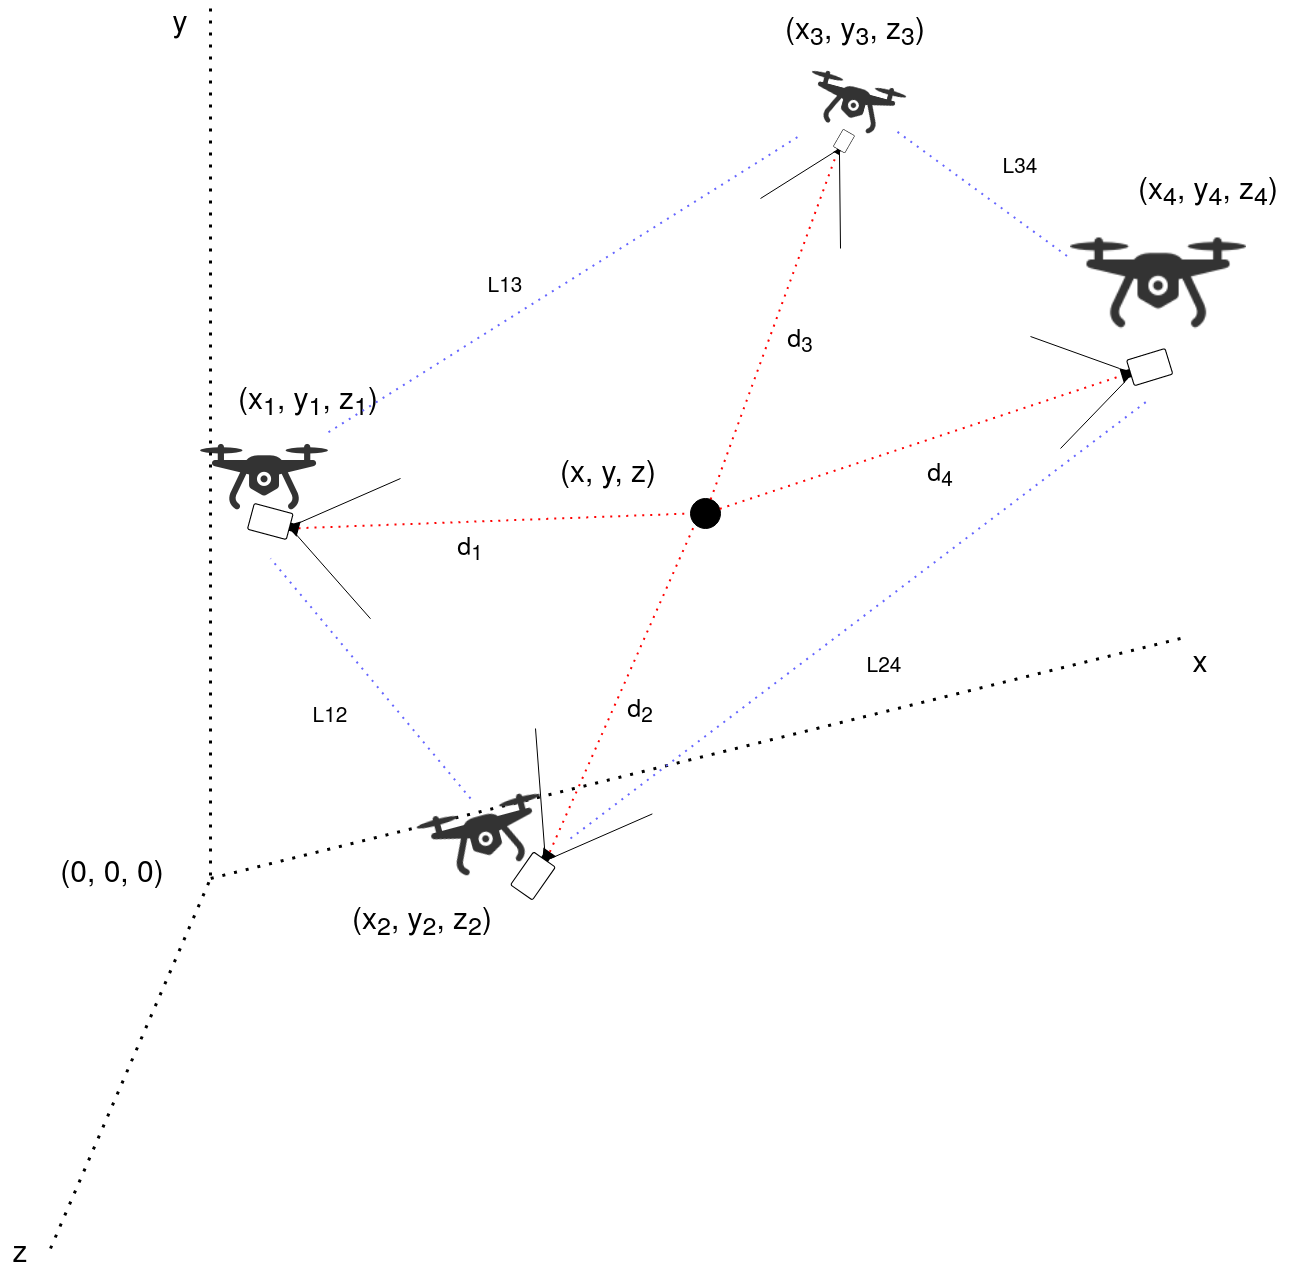
\includegraphics[width=\linewidth]{Images/3dDrones-camera-pose.png}
  \caption{3D drones}
  \label{fig:1}
\end{figure}

\section{APPROACH}


\section{WORK PLAN}
Σε πρώτο επίπεδο θα αποκτηθούν γνώσεις σχετικά με την βιβλιοθήκη OpenCV [], μέσω της οποίας
με οπτικό τρόπο θα εντοπιστεί το αντικείμενο - με βάση τις ιδιότητες του (σχήμα/χρώμα) - ώστε 
να γίνει blob detection

Σε περίπτωση όπου επιτραπεί χρονικά θα γίνει προσπάθεια διόρθωσης των τιμών του 
GPS με RF-based μεθόδων. Πιο συγκεκριμένα με μέτρηση απόστασης μεταξύ των nodes των 
συστήματος σε Ultra wide band, όπως με το πρότυπο IEEE 802.15.4-2011 το οποίο υπόσχεται
ακρίβεια 5-10cm σε εμβέλεια 200m και αυτές οι αποστάσεις να συμβάλουν επίσης στον localization
algorithm.


\begin{figure}[thpb]
  \centering
  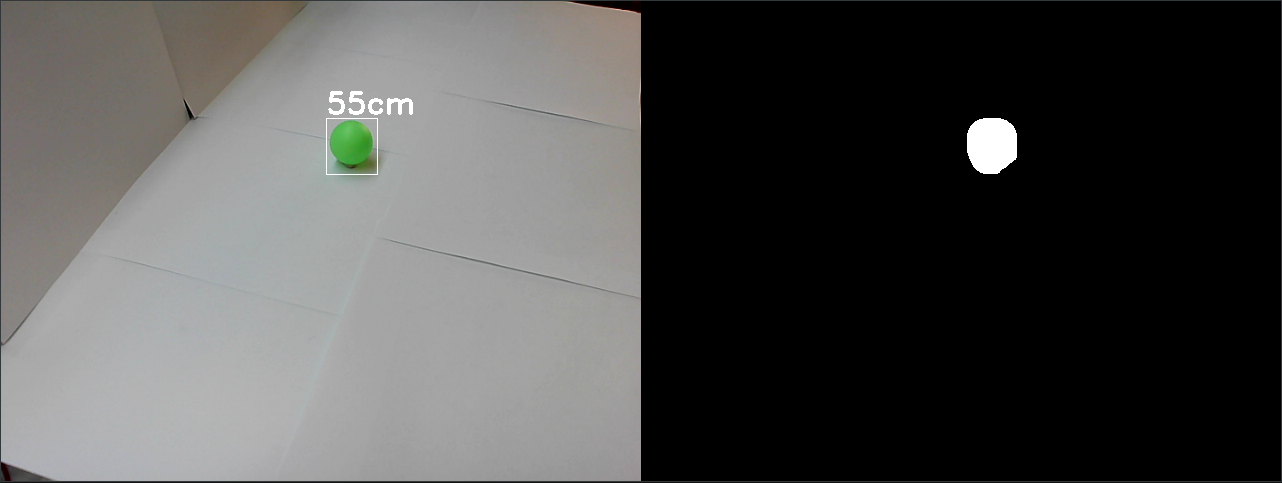
\includegraphics[width=\linewidth]{Images/Thesis-Proposal-shape-color-detection.png}
  \caption{Blob detection - σύμφωνα με το σχήμα/χρώμα - της μπάλας και υπολογισμός της απόστασης της από την κάμερα}
  \label{fig:2}
\end{figure}


\begin{table}[H]
  \caption[]{Raspberry Pi 4 Model B Specifications}
  \label{tab:1}
  \centering
  \begin{tabular}{ll}
      \hline
      \textbf{Feature} & \textbf{Value}  \\
      \hline
          Processor & \Centerstack{Broadcom BCM2711, Quad core Cortex-A72 \\(ARM v8) 64-bit SoC @ 1.5GHz }\\
          Memory & 8GB LPDDR4-3200 SDRAM \\
          Storage & External Micro-SD \\  
          Power & 5V DC (maximum 3A), 5-15Watt \\
          Cost & $\sim$100 €\\
          Weight & 46 grams (without case), 99 grams (with case) \\
          Peripherals & GPIO, I2C, SPI, UART \\
          \hline
  \end{tabular}
\end{table}


\begin{table}[H]
  \caption[]{Jetson Nano Developer Kit Specifications}
  \label{tab:2}
  \centering
  \begin{tabular}{ll}
      \hline
      \textbf{Feature} & \textbf{Value}  \\
      \hline
          CPU & Quad-core ARM Cortex-A57 MPCore processor\\
          GPU & \Centerstack{NVIDIA Maxwell architecture with 128 NVIDIA\\ CUDA® cores} \\
          Memory & 4 GB 64-bit LPDDR4; 25.6 gigabytes/second \\
          Storage & External Micro-SD \\  
          Power & 5V DC, 5-10Watt \\
          Cost & $\sim$120€\\
          Weight & 250 grams (without case)\\
          Peripherals & GPIO, I2C, I2S, SPI, UART \\
          \hline
  \end{tabular}
\end{table}